%%
% The BIThesis Template for Bachelor Graduation Thesis
%
% 北京理工大学毕业设计 (论文) 第二章节 —— 使用 XeLaTeX 编译
%
% Copyright 2020-2023 BITNP
%
% This work may be distributed and/or modified under the
% conditions of the LaTeX Project Public License, either version 1.3
% of this license or (at your option) any later version.
% The latest version of this license is in
%   http://www.latex-project.org/lppl.txt
% and version 1.3 or later is part of all distributions of LaTeX
% version 2005/12/01 or later.
%
% This work has the LPPL maintenance status `maintained'.
%
% The Current Maintainer of this work is Feng Kaiyu.
%%

\chapter{点云配准相关背景知识介绍}
本章将对点云配准的基本理论和相关背景知识进行系统阐述,首先会介绍点云数据的特征,然后会对点云配准的刚体运动和运动参数估计进行介绍。

\section{点云数据}
三维世界中的数据表证有多种类型,如点云数据 (Point Clouds) \cite{leberl2010point} 、三角网格 (Triangle Mesh) \cite{jiang2020local} 、体素 (Voxel Grids) \cite{guan2020voxel} 、深度相机数据 (RGB-D Camera) \cite{cruz2012kinect} 等,可视化数据如图 \ref{fig:3ddata} 所示,本文主要研究的是点云数据,因此本节将对点云数据进行简要介绍。

\begin{figure*}[ht]
    \vspace{-8mm}
    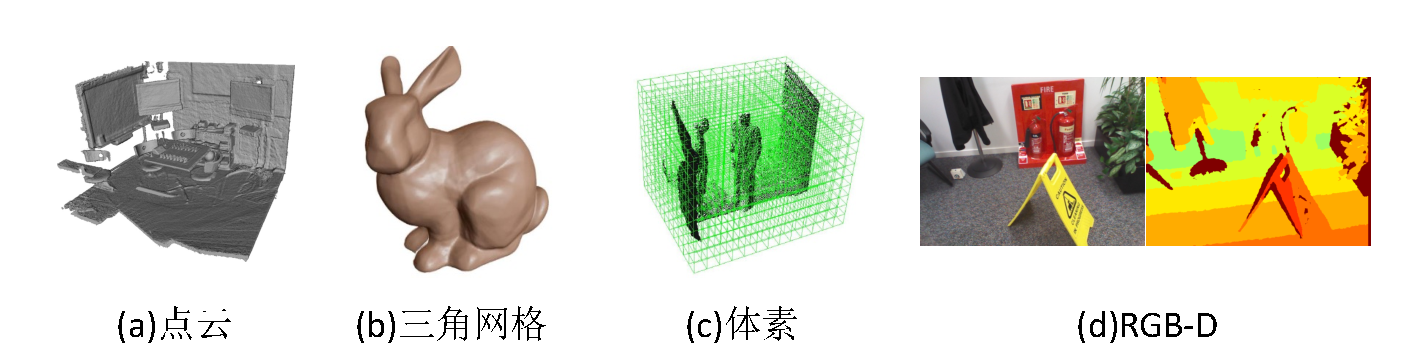
\includegraphics[width=\textwidth]{images/3ddata.pdf}
    \caption{点云、三角网格、体素、深度相机数据可视化示意图}
    \label{fig:3ddata}
    \vspace{-10mm}
\end{figure*}


\subsection{点云数据特点}
点云数据是一种常用的三维数据表征形式,由一系列具有三维坐标 (X, Y, Z) 的点组成。这些点可以通过激光雷达、结构光传感器、多视角立体视觉等方式采集。点云数据具有以下特点:

1. 无序性:点云数据通常是无序的,即点在数据结构中的顺序并不表示它们在空间中的相对位置。这使得处理点云数据时需要额外关注邻域搜索等问题。

2. 不完整性:由于采集设备的视野限制以及物体遮挡等因素,点云数据往往只能捕捉到物体表面的部分信息,无法完整地描述物体的几何结构。

3. 稀疏性:点云数据在空间中分布可能是不均匀的,有些区域可能点密集,而有些区域可能点稀疏。这会对点云处理算法的性能产生影响。

4. 噪声敏感性:点云数据容易受到测量噪声、环境光照等因素的影响。为了提高数据质量,通常需要对点云进行预处理,如滤波、降采样等。

5. 缺乏拓扑信息:点云数据仅包含物体表面的几何信息,不包含拓扑信息。在需要考虑物体结构的应用场景中,点云数据需要进行进一步处理,如重建三角网格或提取骨架结构等。

6. 可扩展性:点云数据可以方便地扩展以包含其他属性信息,如颜色、法向量、强度等。这有助于提高点云处理算法的性能和鲁棒性。

7. 易于处理和存储:由于点云数据直接表示了物体表面的几何信息,其数据结构简单,便于处理和存储。此外,点云数据可以通过各种数据结构 (如KD树、八叉树等) 进行高效的组织和检索。

在应用深度学习算法时,由于点云数据的无序性,深度学习算法,比如全连接层、卷积层等无法直接应用于点云数据。因此,需要对点云数据进行预处理,将其转换为有序的数据表征形式,如三角网格\cite{jiang2020local}、体素\cite{guan2020voxel}等。但是这样的方法会造成空间中很多点的浪费,使得输入的数据变得更加稀疏,使得训练数据变少。PointNet\cite{qi2017pointnet}是一种用于处理点云数据的深度学习网络结构,于2017年首次提出。它是一个端到端的神经网络,可以直接从原始点云数据中学习特征表示。PointNet通过使用对称函数 (如最大池化) 处理输入点云的无序性,同时具有对输入点顺序的不变性。


\subsection{点云特征描述}
三维点云的特征描述,也叫描述子(Descriptor),是一种用于表示点云数据中每个点周围的局部几何特征的向量。描述子捕捉了点云中每个点的几何结构和形状信息,这对于解决诸如点云配准、物体识别、分类和分割等问题至关重要。点云描述子应具有以下特性:鲁棒性、区分性、旋转不变性、尺度不变性和噪声不敏感性。点云描述子对于点云的后处理有着非常巨大的影响,对于不同的任务和数据特征,应该选用合适的描述子来作为网络的预处理。

有许多不同类型的点云描述子,它们根据计算方法和考虑的几何属性而有所不同。以下是一些常见的点云描述子:

1. Spin Images (旋转图像)  \cite{johnson1997spin} :通过在点云中每个点周围投影二维图像来表示局部形状信息。

2. Normal Aligned Radial Features (NARF)  \cite{steder2010narf} :基于局部表面法线的方向和强度来描述点云中的局部特征。

3. Fast Point Feature Histograms (FPFH)  \cite{rusu2009fast} :通过计算每个点周围的点对的几何特征直方图来表示局部特征。

4. Signature of Histograms of Orientations (SHOT)  \cite{salti2014shot} :结合局部点的颜色信息和表面法线分布,为每个点计算描述子。

5. Point Pair Features (PPF)  \cite{deng2018ppfnet} :描述点云中两个点之间的几何关系,PPF 是一个四元组$(\alpha, d, \theta, \phi)$,其中$\alpha$是两点之间的距离,$d$是两点的法向量之差,$\theta$是两点的法线之间的角度,$\phi$是两点的法线在两点之间连线所确定的平面上的角度。PPF特征在处理点云配准问题时具有很高的鲁棒性,因为它仅依赖于点云的几何信息。

\section{刚体运动表示}
刚体运动表示是点云配准任务的最后一个阶段的任务。对于位移来说,常用的是位移向量 (Transition) ;旋转的运动参数有不同的表示形式,如欧拉角\cite{pio1966euler} 、四元数\cite{shoemake1985animating} 、旋转矩阵\cite{horn1954doubly} 、轴角\cite{diebel2006representing} 等。下面我们进行简要介绍。

\subsection{旋转矩阵}
旋转矩阵是一种与向量相乘时旋转向量同时保持其长度的矩阵。所有 $3 \times 3$ 旋转矩阵的特殊正交群表示为 $SO(3)$。因此,如果 $\boldsymbol{R} \in SO(3)$,那么
\begin{equation}
\det (\boldsymbol{R}) = \pm1 \quad \text{且} \quad \boldsymbol{R}^{-1} = \boldsymbol{R}^T
\end{equation}

对于满足 $\det (\boldsymbol{R}) = 1$ 的旋转矩阵,称为正规旋转;对于满足 $\det (\boldsymbol{R}) = -1$ 的旋转矩阵,称为非正规旋转。非正规旋转也称为旋转倒数,由旋转后接反演操作组成。我们将分析限制在正规旋转上,因为非正规旋转不是刚体变换。
我们按如下方式引用旋转矩阵的元素:
\begin{align}
    \boldsymbol{R} &=
    \begin{bmatrix}
    r_1 & r_2 & r_3
    \end{bmatrix} \\
    &=
    \begin{bmatrix}
    r_{11} & r_{12} & r_{13} \\
    r_{21} & r_{22} & r_{23} \\
    r_{31} & r_{32} & r_{33}
    \end{bmatrix}
\end{align}

对于正规旋转矩阵,我们可以使用群的定义来进行更精准的定义。
\begin{equation}
    SO(n) = \{\boldsymbol{R} \in \mathbb{R}^{n \times n} | \boldsymbol{R}^T\boldsymbol{R} = \boldsymbol{I}, \det (R) = 1\}
\end{equation}
其中,$SO(n)$是特殊正交群 (Special Orthogonal Group),这个集合由$n$维空间的旋转矩阵组成。$SO(n)$是一个群,因为它满足群的四个条件:封闭性、结合律、单位元和逆元。$SO(n)$的单位元是 $\boldsymbol{I}$,逆元是 $\boldsymbol{R}^T$。$SO(n)$的元素称为正规旋转矩阵。通过旋转矩阵可以直接描述相机的旋转。

为了描述两个坐标之间的相对旋转,我们假设某个单位正交基 $\boldsymbol{i}, \boldsymbol{j}, \boldsymbol{k}$,并且我们希望将其旋转到另一个正交基 $\boldsymbol{i}', \boldsymbol{j}', \boldsymbol{k}'$。假设对于同一个向量$\boldsymbol{a} = [a_1, a_2, a_3]^T$,在两个坐标系中的表示分别为 $\boldsymbol{a} = a_1\boldsymbol{i} + a_2\boldsymbol{j} + a_3\boldsymbol{k}$ 和 $\boldsymbol{a}' = a_1'\boldsymbol{i}' + a_2'\boldsymbol{j}' + a_3'\boldsymbol{k}'$,根据坐标的定义,有
\begin{equation}
    [\boldsymbol{i}, \boldsymbol{j}, \boldsymbol{k}] \boldsymbol{a} = [\boldsymbol{i}', \boldsymbol{j}', \boldsymbol{k}'] \boldsymbol{a}'
\end{equation}
我们对上述等式同时左成$[\boldsymbol{i}, \boldsymbol{j}, \boldsymbol{k}]^T$,我们可以通过旋转矩阵 $\boldsymbol{R}$ 来表示两个坐标系之间的旋转关系,即
\begin{equation}
    \boldsymbol{a}' = 
    \begin{bmatrix}
    \boldsymbol{i}^T \boldsymbol{i}' & \boldsymbol{i}^T \boldsymbol{j}' & \boldsymbol{i}^T \boldsymbol{k}' \\
    \boldsymbol{j}^T \boldsymbol{i}' & \boldsymbol{j}^T \boldsymbol{j}' & \boldsymbol{j}^T \boldsymbol{k}' \\
    \boldsymbol{k}^T \boldsymbol{i}' & \boldsymbol{k}^T \boldsymbol{j}' & \boldsymbol{k}^T \boldsymbol{k}'
    \end{bmatrix}
    =
    \boldsymbol{R} \boldsymbol{a}
\end{equation}

因为旋转矩阵是正交矩阵,它的逆就可以用来描述一个相反的旋转,按照上面的推到,则有:
\begin{equation}
    \boldsymbol{a} = \boldsymbol{R}^T \boldsymbol{a}' = \boldsymbol{R}^{-1} \boldsymbol{a}'
\end{equation}

在欧式变换中,除了旋转还有平移,将$\boldsymbol{a}$经过一次旋转$\boldsymbol{R}$和平移$\boldsymbol{t}$,最终得到了$\boldsymbol{a}'$,把旋转和平移组合起来,得到:
\begin{equation}
    \boldsymbol{a}' = \boldsymbol{R} \boldsymbol{a} + \boldsymbol{t}
    \label{eq:rotation_translation}
\end{equation}

\subsection{变换矩阵}
在三维空间中,我们可以通过平移和旋转来描述一个刚体的变换。我们将平移和旋转组合起来,得到一个变换矩阵,用来描述一个刚体的变换。假设我们有一个刚体,它的初始位置在原点,我们将它平移到 $\boldsymbol{t}$,然后将它旋转到 $\boldsymbol{R}$,则这个刚体的变换矩阵为:
\begin{equation}
    \boldsymbol{T} = 
    \begin{bmatrix}
    \boldsymbol{R} & \boldsymbol{t} \\
    \boldsymbol{0}^T & 1
    \end{bmatrix}
\end{equation}
将向量改写为齐次形式$\widetilde{\boldsymbol{a}} = [a_1, a_2, a_3, 1]^T = [\boldsymbol{a}, 1]^T$, 那么我们可以将式 \ref{eq:rotation_translation} 重写为:
\begin{equation}
    \widetilde{\boldsymbol{a}}' = \boldsymbol{T} \widetilde{\boldsymbol{a}} = \boldsymbol{R} \boldsymbol{a} + \boldsymbol{t}
\end{equation}  

依靠变换矩阵,我们可以对多次变换的累加进行很简洁的数学表达。假设我们有一个刚体$\boldsymbol{a}$,它的初始位置在原点,我们将它经过 $\boldsymbol{T}_1, \boldsymbol{T}_2$ 两次变换,则这个刚体的最终位置为$\widetilde{\boldsymbol{a}}' = \boldsymbol{T}_1 \boldsymbol{T}_2 \widetilde{\boldsymbol{a}}$。

\subsection{欧拉角}
三次坐标旋转依次可以描述任意旋转。我们考虑三次旋转,其中第一次旋转是关于 $\boldsymbol{k}$ 轴的角度 $\psi$,第二次旋转是关于 $\boldsymbol{j}$ 轴的角度 $\theta$,第三次旋转是关于 $\boldsymbol{i}$ 轴的角度 $\phi$,如图 \ref{fig:rotation} (a, b ,c)所示。为了简化符号,我们将这些角度排列成一个三维向量,称为欧拉角向量,定义为 
\begin{equation}
    \boldsymbol{u} := [\phi, \theta, \psi]^T
\end{equation}
将欧拉角向量映射到其对应的旋转矩阵的函数,$\boldsymbol{R}_{ijk} : \mathbb{R}^3 \to SO(3)$,定义为
\begin{equation}
    \boldsymbol{R}_{ijk}(\phi, \theta, \psi) := \boldsymbol{R}_i(\phi)\boldsymbol{R}_j(\theta)\boldsymbol{R}_k(\psi)
\end{equation}
与一般情况相同,如果 $\boldsymbol{z} \in \mathbb{R}^3$ 是世界坐标系中的一个向量,$\boldsymbol{z}_0 \in \mathbb{R}^3$ 是以体固定坐标表示的相同向量,那么以下关系成立:
\begin{align}
    \boldsymbol{z}_0 = \boldsymbol{R}_{ijk}(\boldsymbol{u}) \boldsymbol{z} \\
    \boldsymbol{z} = \boldsymbol{R}_{ijk}(\boldsymbol{u})^T \boldsymbol{z}_0
\end{align}
也就是说,欧拉角并不是定义在三维线性空间的群,欧拉角的相互转换需要借助旋转矩阵来进行表达。

\begin{figure}
    \centering
    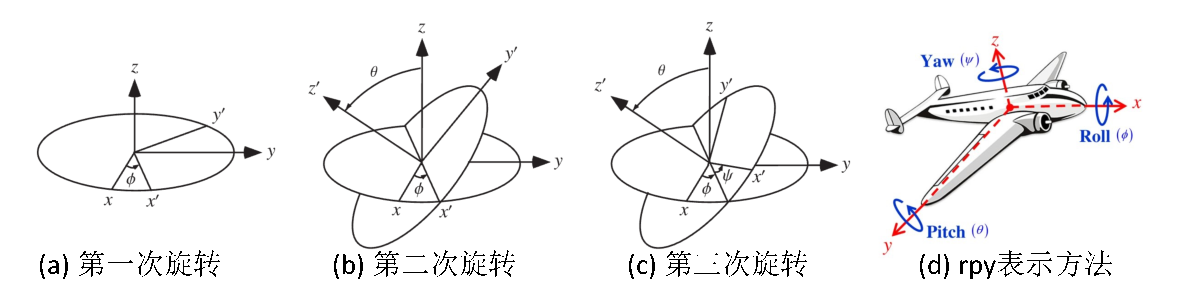
\includegraphics[width=\textwidth]{images/rotation.pdf}
    \caption{欧拉角旋转表示}
    \label{fig:rotation}
    \vspace{-0.5cm}
\end{figure}

在自动化或者航空航天领域比较常用的欧拉角的分解方式是 $Z-Y-X$,也就是说,先绕 $z$ 轴旋转 $\psi$ 角,然后绕 $y$ 轴旋转 $\theta$ 角,最后绕 $x$ 轴旋转 $\phi$ 角。这种分解方式也被称为航空分解 (Aerospace decomposition) ,通常这种方式中的$Z-Y-X$会被称为“偏航 - 俯仰 - 旋转 (yaw - pitch - roll)”。在这种分解方式中,欧拉角向量的顺序是 $\boldsymbol{u} = [\psi, \theta, \phi]^T$,如图 \ref{fig:rotation} (d)所示。

欧拉角的一个缺点是会碰到著名的万象锁问题\cite{vsenk2006rotation} ,也就是说,当 $\theta = \pm \frac{\pi}{2}$ 时,旋转矩阵 $\boldsymbol{R}_{ijk}(\boldsymbol{u})$ 的值会变成奇异的。理论上可以证明,只要想要用3个数来表达三位旋转时,基本都会碰到奇异性问题\cite{stuelpnagel1964parametrization} 。由于这种原理,欧拉角不适用于迭代和插值,在传统的SLAM中和深度学习中几乎都不会是用这种方式来进行迭代,但是欧拉角对于人机交互是友好的。

\subsection{四元数}
旋转矩阵使用了9个未知数来描述3自由度的旋转,这在数学表达上具有冗余性了;欧拉角使用了3个未知数来描述3自由度的旋转,在数学表达上是紧凑的,但是具有奇异性。因为我们找不到不带奇异性,且使用3个未知数的方法来描述3维旋转的描述方式\cite{stuelpnagel1964parametrization} 。这个性质,可以类比于用两个坐标描述地球表面 (二维流形) 上的点,我们可以使用经纬度来描述地球表面上的点,但是在极点处,经纬度的表达就会出现奇异性,即纬度为$\pm 90^{\circ}$时,经度无意义。

三位旋转是一个三维流形,因此,为了最优平衡无奇异性和数学表达的紧凑性,我们需要引入一个新的数学工具来描述3自由度的旋转,这个数学工具就是四元数。四元数是Hamilton找到的一种超复数,它在数学形式上既是紧凑的,又是非奇异的。四元数的定义如下:
\begin{equation}
    \boldsymbol{q} = q_0 + q_1 i + q_2 j + q_3 k
\end{equation}
其中,$q_0, q_1, q_2, q_3 \in mathbb{R}$,$i, j, k$ 是四元数的三个虚数单位,满足如下关系:
\begin{equation}
    \left\{
    \begin{aligned}
        &i^2 = j^2 = k^2 = ijk = -1, \\
        &ij = k, jk = i, ki = j, \\
        &ji = -k, kj = -i, ik = -j
    \end{aligned}
    \right.
\end{equation}
假设某个旋转是绕着单位向量 $\boldsymbol{u} = [u_x, u_y, u_z]^T$ 旋转 $\theta$ 角,那么这个旋转可以用四元数来表示为:
\begin{equation}
    \boldsymbol{q} = \cos \frac{\theta}{2} + \sin \frac{\theta}{2} (u_x i + u_y j + u_z k)
\end{equation}
同时,我们也可以从单位四元数种计算出对应的旋转轴和旋转角:
\begin{equation}
    \left\{
    \begin{aligned}
        &\theta = 2 \arccos q_0, \\
        &u_x = \frac{q_1}{\sin \frac{\theta}{2}}, u_y = \frac{q_2}{\sin \frac{\theta}{2}}, u_z = \frac{q_3}{\sin \frac{\theta}{2}}
    \end{aligned}
    \right.
\end{equation}

因为四元数是定义在复向量空间中而非旋转流形中,并且四元数没有死锁的特性,所以在深度学习的梯度下降算法中,常常用四元数作为回归的目标。并且,因为三维流形的性质,我们在四元数中同乘一个常数,可以得到相同的旋转,即$[q_0, q_1, q_2, q_3] \iff k[q_0, q_1, q_2, q_3]$。由于这个性质,在回归任务中,我们通常回归单位四元数,即$\sum_0^3 q_i^2 = 1$。

{\bf 用四元数表示旋转。} 用四元数同样也可以表达对一个点的旋转,假设一个空间中的三维坐标点为$\boldsymbol{a} = [x, y, z] \in \mathbb{R}^3$。以及一个旋转轴$\boldsymbol{n}$和旋转角$\theta$,这个点绕着旋转轴旋转$\theta$角后的坐标为$\boldsymbol{a}'$,则:
\begin{equation}
    \boldsymbol{p}' = \boldsymbol{Rp} = \boldsymbol{qpq}^{-1}
\end{equation}
其中,$\boldsymbol{q} = [\cos \frac{\theta}{2}, \boldsymbol{n} \sin \frac{\theta}{2}]$。


\section{运动学参数估计}
\subsection{基于奇异值分解的线性代数求解}
奇异值分解\cite{levinson2020analysis} (Singular Value Decomposition, SVD) 是线性代数中一种重要的矩阵分解,在信号处理、计算机视觉、运动估计中有着非常广泛的运用。下面,我们对奇异值分解的线性代数部分进行简要介绍。

奇异值分解对一个矩形数据矩阵 (定义为$\boldsymbol{A}$,其中$\boldsymbol{A}$是一个$n \times p$矩阵) 进行处理,其中n行代表观察值,p列代表变量。SVD定理如下:
\begin{equation}
\boldsymbol{A}_{n \times p} = \boldsymbol{U}_{n \times n} \boldsymbol{S}_{n \times p} \boldsymbol{V}^T_{p \times p}
\end{equation}
其中
\begin{align}
    \boldsymbol{U}^T \boldsymbol{U} = \boldsymbol{I}_{n \times n} \\
    \boldsymbol{V}^T \boldsymbol{V} = \boldsymbol{I}_{p \times p}
\end{align}

即$\boldsymbol{U}$和$\boldsymbol{V}$是正交的。$\boldsymbol{U}$的列是左奇异向量 (观察值系数向量) ;$\boldsymbol{S}$ (与$\boldsymbol{A}$的维度相同) 具有奇异值,并且是对角的 (模振幅) ;$\boldsymbol{V}^T$的行是右奇异向量 (变量水平向量)。SVD表示了原始数据在协方差矩阵为对角线的坐标系中的扩展。

计算SVD包括寻找$\boldsymbol{A} \boldsymbol{A}^T$和$\boldsymbol{A}^T \boldsymbol{A}$的特征值和特征向量。$\boldsymbol{A}^T \boldsymbol{A}$的特征向量构成$\boldsymbol{V}$的列,$\boldsymbol{A} \boldsymbol{A}^T$的特征向量构成$\boldsymbol{U}$的列。此外,$\boldsymbol{S}$中的奇异值是来自$\boldsymbol{A} \boldsymbol{A}^T$或$\boldsymbol{A}^T \boldsymbol{A}$的特征值的平方根。奇异值是$\boldsymbol{S}$矩阵的对角线条目,并按降序排列。奇异值总是实数。如果矩阵$\boldsymbol{A}$是实数矩阵,那么$\boldsymbol{U}$和$\boldsymbol{V}$也是实数。

奇异值分解 (SVD) 在点云配准问题中也具有重要应用。点云配准是将两个或多个点云数据集合并为一个统一坐标系的过程。在这种情况下,我们的目标是找到一个最优的刚体变换,包括旋转和平移,使得两个点云之间的距离最小化。

假设我们有两个点云数据集$\boldsymbol{P}$和$\boldsymbol{Q}$,每个点云包含$n$个点。我们首先计算两个点云的质心$\boldsymbol{p}_c$和$\boldsymbol{q}_c$,然后将点云平移到原点。接下来,我们计算点云$\boldsymbol{P}$和$\boldsymbol{Q}$之间的距离矩阵$\boldsymbol{H}$,其中$\boldsymbol{H}=\boldsymbol{P}^T\boldsymbol{Q}$。

在这种情况下,我们可以使用SVD来求解最优的旋转矩阵$\boldsymbol{R}$,使得两个点云之间的距离最小化。具体来说,我们对距离矩阵$\boldsymbol{H}$进行奇异值分解:

\begin{equation}
\boldsymbol{H} = \boldsymbol{U} \boldsymbol{S} \boldsymbol{V}^T
\end{equation}

然后,我们计算旋转矩阵$\boldsymbol{R}$:

\begin{equation}
\boldsymbol{R} = \boldsymbol{U} \boldsymbol{V}^T
\end{equation}

如果$\boldsymbol{R}$是一个不合适的旋转矩阵 (即$\det(\boldsymbol{R})\neq 1$) ,我们可以通过修改$\boldsymbol{S}$矩阵来修复它。具体而言,我们将$\boldsymbol{S}$的最小奇异值设为$-1$,然后重新计算旋转矩阵$\boldsymbol{R}$。

最后,我们可以计算最优的平移向量$\boldsymbol{t}$:

\begin{equation}
\boldsymbol{t} = \boldsymbol{q}_c - \boldsymbol{R} \boldsymbol{p}_c
\end{equation}

通过应用旋转矩阵$\boldsymbol{R}$和平移向量$\boldsymbol{t}$,我们可以将点云$\boldsymbol{P}$对齐到点云$\boldsymbol{Q}$,从而实现点云配准。

\subsection{基于Levenberg-Marquardt算法的非线性优化求解}
在数学和计算领域,Levenberg-Marquardt算法 (LMA或简称LM) \cite{levenberg1944method} ,也称为阻尼最小二乘法 (DLS) ,用于求解非线性最小二乘问题。这些最小化问题尤其出现在最小二乘曲线拟合中。LMA在高斯-牛顿算法 (GNA) 和梯度下降法之间进行插值。LMA比GNA更稳健,这意味着在许多情况下,即使它从距离最终最小值非常远的地方开始,也能找到解决方案。对于行为良好的函数和合理的初始参数,LMA往往比GNA慢。LMA也可以被视为使用信任区域方法的高斯-牛顿算法。

需要LM算法求解的问题被称为非线性最小二乘最小化问题。这意味着要最小化的函数具有以下特殊形式:

\begin{equation}
f(x) = \frac{1}{2} \sum_{j=1}^{m} r_j^2(x)
\end{equation}

其中 $x = (x_1, x_2, \dots, x_n)^T$ 是一个向量,每个 $r_j$ 是一个从 $\mathbb{R}^n$ 到 $\mathbb{R}$ 的函数。$r_j$ 被称为残差,并且假定 $m \geq n$。

为了简化问题,我们用残差向量 $r : \mathbb{R}^n \rightarrow \mathbb{R}^m$ 来表示 $f$,定义为:

\begin{equation}
r(x) =
\begin{bmatrix}
r_1(x) \
r_2(x) \
\cdots \
r_m(x)
\end{bmatrix}
\end{equation}

现在,$f$ 可以重写为 $f(x) = \frac{1}{2} ||r(x)||^2$。$f$ 的导数可以用相对于 $x$ 的 $r$ 的雅可比矩阵 $J(x)$ 来表示,定义为 $J(x) = \frac{\partial r_j}{\partial x_i}$,其中 $1 \leq j \leq m$,$1 \leq i \leq n$。

首先考虑线性情况,其中每个 $r_i$ 函数都是线性的。在这里,雅可比矩阵是常数,我们可以将 $r$ 表示为空间中的超平面,这样 $f$ 给出二次型:

\begin{equation}
f(x) = \frac{1}{2} ||Jx - r_0||^2
\end{equation}

我们还得到 $\nabla f(x) = J^T(Jx - r_0)$ 和 $\nabla^2 f(x) = J^TJ$。通过将 $\nabla f(x) = 0$ 求解最小值,我们得到 $x_\text{min} = (J^TJ)^{-1}J^Tr$,这是一组无约束优化问题的解。

回到一般的非线性情况,我们有:

\begin{equation}
\nabla f(x) = J(x)^T r(x)
\label{eq:grad}
\end{equation}

\begin{equation}
\nabla^2 f(x) = J(x)^TJ(x) + \sum_{j=1}^{m} r_j(x) \nabla^2 r_j(x)
\label{eq:hessian}
\end{equation}

最小二乘问题的独特属性是,给定雅可比矩阵 $J$,如果可以将 $r_j$ 用线性函数近似 ($\nabla^2 r_j(x)$ 较小) 或残差 $r_j(x)$ 本身较小,我们可以实质上免费获得海森矩阵 ($\nabla^2 f(x)$) 。在这种情况下,海森矩阵简化为:

\begin{equation}
\nabla^2 f(x) = J(x)^T J(x)
\label{eq:hessian_approx}
\end{equation}

这与线性情况相同。这里通常使用的近似是在解附近的 $r_i$ 近似线性,这样 $\nabla^2 r_j(x)$ 较小。还要注意,只有在残差较小时,式 \ref{eq:hessian_approx} 才有效。对于大残差问题,不能使用二次近似求解\cite{李娇娇2022基于深度学习的} 。

考虑到点云配准问题,我们可以将 Levenberg-Marquardt 算法应用于点云之间的非线性最小二乘优化问题。在这种情况下,我们寻求点云对应度量的最小距离,同时考虑旋转和平移变换。通过迭代地优化变换参数,Levenberg-Marquardt 算法可以在点云配准问题中找到一个稳定的解决方案。点云对应度量之间的误差主要有点到点 (point-to-point) 、点到面 (point-to-plane) 、面到面 (plane-to-plane) 这几类方式。如图 \ref{fig:point2plane} 所示,我们以最小化点到面距离为例,来说明 Levenberg-Marquardt 算法的求解过程。

\begin{figure}[htbp]
    \centering
    \vspace{-0.5cm}
    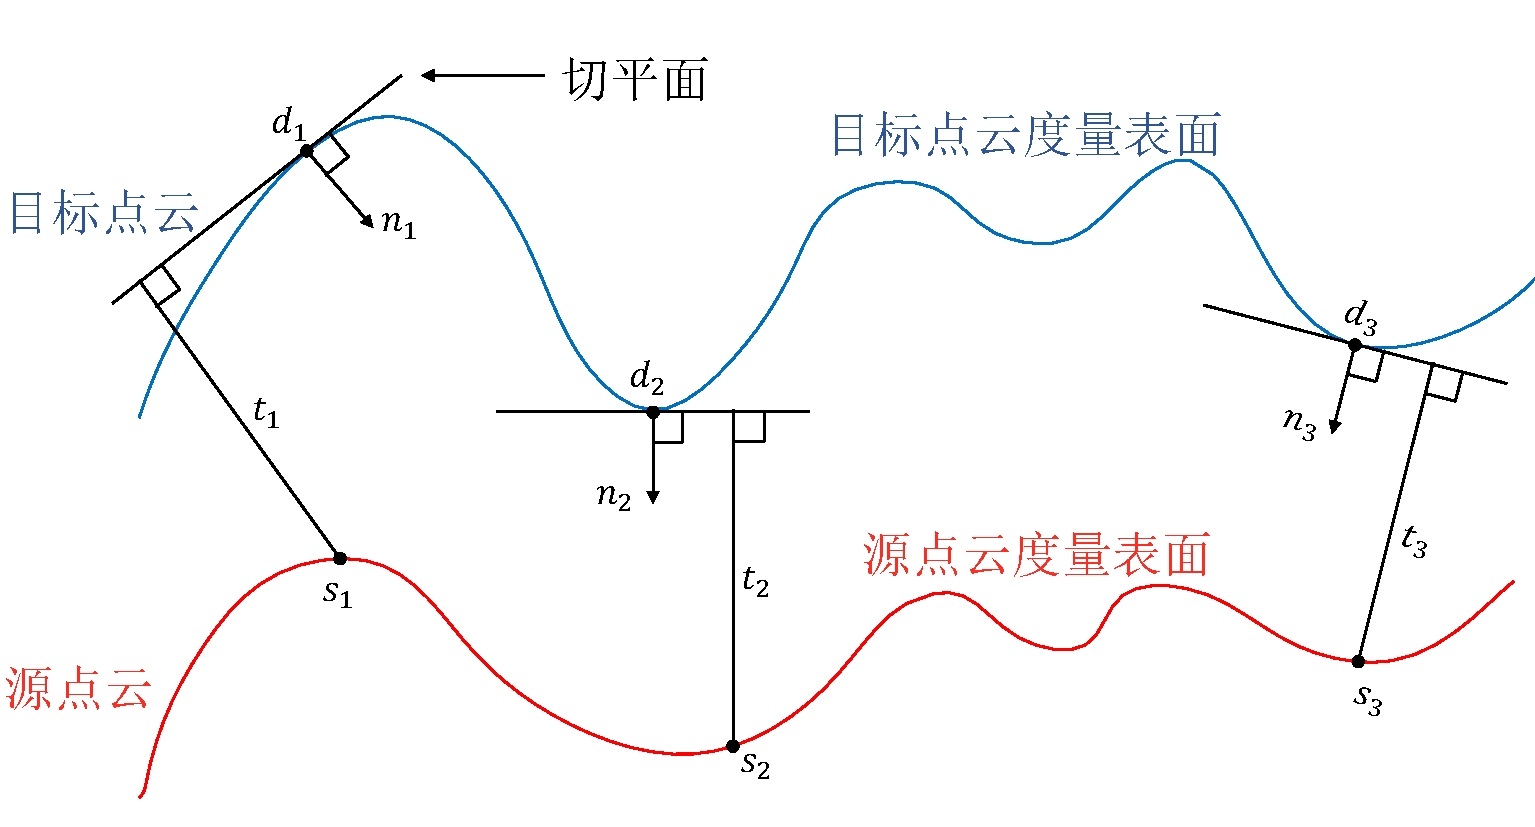
\includegraphics[width=0.8\textwidth]{images/LM_point2plane.pdf}
    \caption{最小化点到面距离示意图}
    \label{fig:point2plane} 
    \vspace{-1.5cm}
\end{figure}

在刚体运动参数估计任务中,LM 算法的关键步骤包括:

 (1) 在运动前的点云数据中找到特征点 $\boldsymbol{p}_i$ 和运动后的点云数据中对应的特征点 $\boldsymbol{q}_j$ 以及特征面 $\boldsymbol{S}_l$;

 (2) 计算特征点 $\boldsymbol{p}_i$ 到特征面 $\boldsymbol{S}_l$ 的欧氏距离 $d_e$;

 (3) 基于特征点到特征面的距离度量,构建匹配对的约束关系:
\begin{equation}
f(\boldsymbol{p}_i, \boldsymbol{T}) = d_e
\end{equation}
其中,$\boldsymbol{T}$ 代表刚体运动变换参数。

利用 LM 非线性优化方法,估计位姿变换矩阵:
\begin{equation}
\hat{\boldsymbol{T}} = \boldsymbol{T} - (\boldsymbol{J}^T \boldsymbol{J} + \lambda \boldsymbol{I})^{-1} \boldsymbol{J}^T f
\label{eq:LM}
\end{equation}
通过链式法则计算雅可比矩阵 (Jacobian Matrix):
\begin{equation}
\boldsymbol{J} = \frac{\partial f}{\partial \boldsymbol{T}} = \frac{\partial f}{\partial \boldsymbol{p}_i} \frac{\partial \boldsymbol{p}_i}{\partial \boldsymbol{T}}
\end{equation}
将雅可比矩阵带入公式 \ref{eq:LM},可以求解刚体运动变换参数 $\boldsymbol{T}$。

 (4) 检查变换参数是否为最优估计,如果满足以下条件:
\begin{equation}
0 < \frac{f(\boldsymbol{p}_i, \hat{\boldsymbol{T}}) - f(\boldsymbol{p}_i, \boldsymbol{T})}{|f(\boldsymbol{p}_i, \boldsymbol{T})|} < T_d
\end{equation}
则当前变换参数为最优估计。否则,调整阻尼因子 $\lambda$,继续迭代求解最优变换参数。其中,$T_d$ 是距离阈值。

 (5) 将求解得到的最优变换参数应用于运动前的特征点 $\boldsymbol{p}_i$,得到 $\boldsymbol{q}'_j$,如果满足以下条件:
\begin{equation}
|\boldsymbol{p}_i - \boldsymbol{q}_j| > |\boldsymbol{p}_i - \boldsymbol{q}'_j|
\end{equation}
则认为 $\boldsymbol{q}_j$ 是点 $\boldsymbol{p}_i$ 的最佳匹配点。否则,减小阻尼因子 $\lambda$,继续迭代求解最优匹配点对。如果达到最大迭代次数仍未找到最优匹配点对,将点 $\boldsymbol{p}_i$ 视为噪点并从原始点云数据中剔除,继续处理其他特征点。

总之,使用 LM 算法进行点云配准的过程可以分为以下几个步骤:\\
1. 在运动前后的点云数据中提取特征点和特征面;\\
2. 计算特征点之间的欧氏距离并建立约束关系;\\
3. 使用 LM 算法进行非线性优化,求解刚体运动变换参数;\\
4. 根据求解结果判断当前变换参数是否为最优估计;如非最优,调整阻尼因子并继续迭代;\\
5. 应用求解得到的最优变换参数,寻找最佳匹配点对;\\
6. 若达到最大迭代次数仍未找到最优匹配点对,将当前特征点视为噪点并剔除,继续处理其他特征点。

\section{小结}
本章主要介绍了点云配准任务的基础知识,包括点云数据的特点,运动学表达和刚体运动参数估计方法。主要介绍了两种最常用的点云配准求解刚体运动最优变换参数的方法,一个是基于奇异值分解 (SVD) 的线性代数求解方法,一个是基于Levenberg-Marquardt算法的非线性优化求解。